\documentclass[10pt,twocolumn,letterpaper]{article}
\usepackage[T1]{fontenc}
\usepackage{newtxtext,newtxmath}
\usepackage[letterpaper,top=1in,bottom=1in,left=0.75in,right=0.75in,columnsep=0.3125in]{geometry}
\usepackage{graphicx,booktabs,amsmath,multirow,xcolor,microtype,enumitem}
\usepackage[font=small,labelfont=bf,skip=4pt]{caption}
\usepackage[colorlinks=true,linkcolor=blue!50!black,citecolor=blue!50!black,urlcolor=blue!50!black]{hyperref}
\usepackage[capitalise,noabbrev]{cleveref}
\usepackage{tikz}
\usetikzlibrary{positioning,arrows.meta,calc}
\graphicspath{{figs/}}
\setlist{itemsep=1pt,topsep=2pt,leftmargin=1.2em}
\newcommand{\pts}{\,pts}
\newcommand{\etal}{et~al.}
\newcommand{\ndom}{\mathrm{ndom}}
\definecolor{acc}{HTML}{2A78D6}

\title{\Large\bf Is Attribute-Based Person Retrieval on Unseen Cameras\\ a Calibration Problem?}
\author{Anonymous authors\\ UPAR Challenge 2027, Track 2 technical report}
\date{}

\begin{document}
\maketitle

\begin{abstract}
Attribute-based person retrieval ranks gallery images against a 40-attribute query, and on unseen cameras it has resisted improvement: in the two previous UPAR challenges no team beat the organizers' baseline. The organizers attributed this to recognizers whose confidences become miscalibrated on new domains. We test that hypothesis on three held-out datasets with 48 trained recognizers. First, the scoring rule matters more than any recognizer change we tried. The standard L1 score treats one confident error like many small doubts, whereas the log-likelihood of the exact query does not, and it raises mADM by 3.7--9.1 points in every one of the 48 runs. Second, under this score the hypothesis is half right. Recalibrating each attribute with the held-out labels would add 1.8--5.7 points depending on the dataset, but 81--97\% of that miscalibration is already present on the source datasets, and recalibration fitted there lowers held-out mADM in 47 of 48 runs. Swapping the two parameters of the fitted maps locates the failure: the per-attribute scale transfers across domains, the per-attribute bias does not. Third, what does transfer is a better training signal. A group cross-entropy over mutually exclusive attributes improves mADM in all eight paired comparisons, on PETA by removing most of the extra held-out miscalibration, and distillation improves refinement in a way that grows with training length. Thresholded accuracy and AUC do not predict any of this within one encoder family, but held-out likelihood does (Spearman $-0.86$). The final system scored 0.6365 mADM on the hidden test set.
\end{abstract}

%=====================================================================
\section{Introduction}

Searching video for ``an adult man in a red jacket and grey trousers, with a backpack'' needs no photograph of the person, only an agreed attribute vocabulary~\cite{upar}. The standard recipe runs an attribute recognizer on every gallery image and compares its probabilities with the binary query vector. The UPAR challenge evaluates this recipe on cameras absent from training, and the results have been poor: in 2023 and 2024 the organizers' baseline was not beaten on this task~\cite{upar23,upar24}. The organizers suggested that strong recognizers produce miscalibrated confidences on new domains~\cite{upar24}.

This suggestion makes a testable prediction. If miscalibration is the bottleneck, then correcting it should recover much of the lost retrieval quality, and the domain shift should be what creates it. We test both parts with an oracle that recalibrates each attribute using the held-out labels, and by comparing calibration on the source and held-out datasets. Before we can do so we must fix the scoring rule, because the baseline L1 score is insensitive to the very property under test.

Our contributions are:
\begin{itemize}
\item We show that ranking by the log-likelihood of the exact query, a direct-attribute-prediction score~\cite{dap}, beats the baseline L1 distance in all 48 runs on three held-out datasets (\cref{sec:score}).
\item We show that under this score, held-out likelihood predicts retrieval within an encoder family, whereas AUC and thresholded accuracy do not (\cref{sec:select}).
\item We separate calibration from refinement on held-out data, and find that miscalibration is real but mostly not caused by the domain shift, and that its non-transferable part is a per-attribute bias (\cref{sec:calib}).
\item We identify training changes that improve held-out retrieval and say which part of the likelihood each one improves (\cref{sec:train}).
\end{itemize}

%=====================================================================
\section{Related Work}

\paragraph{Attribute-based retrieval.} Ranking by attributes predates deep learning: Vaquero~\etal\ searched surveillance video by facial and clothing attributes~\cite{vaquero}, Siddiquie~\etal\ ranked images for multi-attribute queries~\cite{siddiquie}, and direct attribute prediction (DAP)~\cite{dap} scores a class by the product of per-attribute posteriors. The UPAR baseline~\cite{upar} instead ranks by the L1 distance between query and probabilities. Specker and Beyerer proposed a calibrated, weighted, distribution-based distance~\cite{specker21} and later argued for balanced recognizers~\cite{specker23}. Our score is the DAP score applied to a single attribute vector; what is new is the evidence about which recognizer property it rewards on unseen domains.

\paragraph{Proper scores and their decomposition.} Log-loss is a strictly proper scoring rule~\cite{gneiting}. Its expected value splits into a calibration term and a refinement term~\cite{degroot,brocker}; Kull and Flach~\cite{kull} give the decomposition used here, with calibration measured by the loss that a recalibration map can remove. We use the word refinement as they do, not sharpness, which Gneiting~\etal\ define as the concentration of the predictive distribution~\cite{gneitingsharp}.

\paragraph{Calibration under shift.} Temperature scaling removes most in-distribution miscalibration~\cite{guo}, but calibration fitted on source data degrades under dataset shift~\cite{ovadia}. Label smoothing changes the confidence of a network's outputs~\cite{muller}. We measure how much of the held-out miscalibration is already present on the source datasets, which these works do not separate.

\paragraph{Distillation.} Knowledge distillation transfers soft predictions~\cite{hinton}, and it becomes stronger with consistent inputs and long schedules, called function matching~\cite{patient}. Our companion Track~1 report studies the teachers and their effect on ranking~\cite{track1}; here we only measure the retrieval-specific consequences.

%=====================================================================
\section{Task, Metric, Protocol and System}
\label{sec:task}

\paragraph{Task.} Images come from the UPAR re-annotations of PA100k~\cite{pa100k}, Market1501~\cite{market} and PETA~\cite{peta}, with 40 binary attributes. Every distinct label vector in a gallery becomes a query $q\in\{0,1\}^{40}$, and an image matches when all 40 labels agree. The program returns a score for every query--image pair.

\paragraph{mADM.} Let $\mathrm{dom}(q,g)$ be the fraction of attributes on which image $g$ agrees with $q$, normalized per query as
\begin{equation}
\ndom(q,g)=\max\Big(0,\tfrac{\mathrm{dom}(q,g)-\overline{\mathrm{dom}}_q}{\max_{g'}\mathrm{dom}(q,g')-\overline{\mathrm{dom}}_q}\Big),
\end{equation}
where $\overline{\mathrm{dom}}_q$ is the gallery mean. With $r_1<\dots<r_R$ the ranks of the $R$ exact matches,
\begin{equation}
\mathrm{ADM}(q)=\frac1R\sum_{m=1}^{R}P(r_m),\qquad P(r)=\frac1r\sum_{j\le r}\ndom(q,g_{(j)}),
\end{equation}
and mADM averages over queries. ADM is average precision in which every image in the top $r$ earns its degree of match instead of 0 or 1. The exact matches decide where the list is evaluated, and the near-misses above them earn partial credit. On PETA the mean dom of a query is about 0.82, so an image wrong on one attribute earns 0.86, wrong on two earns 0.72, and wrong on eight or more earns nothing. We report differences in points (pts), where 1\pts{} is 0.01 mADM.

\paragraph{Protocol.} We train on two datasets and rank the validation gallery of the third (leave-one-dataset-out, LODO). PETA is the main held-out domain, with 1{,}763 queries, 61\% of which have a single match. Market1501 and PA100k serve as checks. The PA100k fold is unusual: holding out PA100k leaves only 18.7k training images, five times fewer than the other folds, and its models are the worst calibrated (\cref{tab:calib}). We analyze 48 runs with saved held-out logits: 41 on PETA, 5 on Market1501 and 2 on PA100k.

\paragraph{Noise model.} Three pairs of runs differ only in the seed or are identical configurations; their mADM differs by 0.08, 0.16 and 0.33\pts, a pooled standard deviation of 0.15\pts. Resampling queries gives a paired standard error of 0.24--0.29\pts\ for two models on the same gallery. We treat differences below about 0.3\pts\ as ties.

\paragraph{System.} \Cref{fig:pipe} shows the submitted system. The recognizer is a DINOv3 ViT-B/16~\cite{dinov3} at $256\times128$ with one learned query per attribute that cross-attends to the image tokens~\cite{track1}. A ViT-B is what the challenge's CPU time limit allows without risk; Track~1 describes the trade-off. The probabilities are used without offsets or temperature. \Cref{sec:train} describes the three training choices: label smoothing, group cross-entropy and distillation.

\begin{figure*}[t]
\centering
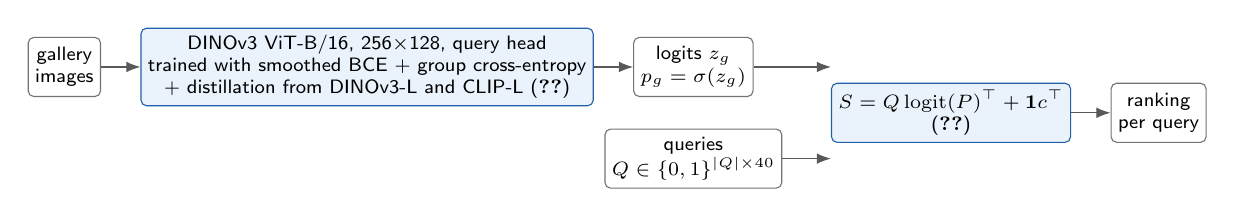
\begin{tikzpicture}[font=\sffamily\scriptsize, node distance=3.5mm and 5mm,
  box/.style={draw=black!55, rounded corners=2pt, fill=white, align=center, minimum height=7.5mm, inner sep=2.5pt},
  hl/.style={box, fill=acc!10, draw=acc!80!black}, arr/.style={-{Latex[length=1.8mm]}, black!65}]
\node[box] (g) {gallery\\ images};
\node[hl, right=of g] (m) {DINOv3 ViT-B/16, 256$\times$128, query head\\ trained with smoothed BCE + group cross-entropy\\ + distillation from DINOv3-L and CLIP-L (\cref{sec:train})};
\node[box, right=of m] (p) {logits $z_g$\\ $p_g=\sigma(z_g)$};
\node[box, below=4mm of p] (q) {queries\\ $Q\in\{0,1\}^{|Q|\times40}$};
\node[hl, right=8mm of $(p.east)!0.5!(q.east)$] (s) {$S=Q\,\mathrm{logit}(P)^{\top}+\mathbf 1c^{\top}$\\ (\cref{eq:ll})};
\node[box, right=of s] (o) {ranking\\ per query};
\draw[arr] (g)--(m); \draw[arr] (m)--(p); \draw[arr] (p.east)--(s.west |- p.east); \draw[arr] (q.east)--(s.west |- q.east); \draw[arr] (s)--(o);
\end{tikzpicture}
\caption{Submitted system. The recognizer runs once per gallery image, and scoring all query--image pairs is one matrix product.}
\label{fig:pipe}
\end{figure*}

%=====================================================================
\section{Scoring by the Likelihood of the Exact Query}
\label{sec:score}

The baseline score $s_{L1}(q,g)=-\sum_k|q_k-p_{gk}|$ is minus the expected number of wrong attributes, so it ignores how those errors are distributed. Consider an image whose 40 attributes are each 90\% likely to agree with the query, and another with 36 certain agreements and 4 certain disagreements. Both score $-4$, yet only the first can be an exact match.

Since exact matches decide where ADM is evaluated, a natural alternative is the probability that the image matches exactly. The probability ranking principle~\cite{prp} makes this the optimal score for retrieving exact matches if the probabilities are correct. Assuming attributes are independent given the image, its logarithm is
\begin{equation}
\begin{aligned}
s_{LL}(q,g)&=\sum_{k}\big[q_k\log p_{gk}+(1-q_k)\log(1-p_{gk})\big]\\
&=q^\top\!\log\tfrac{p_g}{1-p_g}+\textstyle\sum_k\log(1-p_{gk}),
\end{aligned}
\label{eq:ll}
\end{equation}
which is one matrix product plus a per-image bias. ADM also credits near-misses, so the exact-match probability is not the ADM-optimal score. We tested the obvious correction, adding the expected ndom of each image computed exactly from the Poisson-binomial distribution of errors (\cref{app:impl}): it adds 0.29\pts\ on PETA, about one standard error. The exact-match term therefore carries the metric.

\begin{table}[t]
\centering\small
\setlength{\tabcolsep}{3pt}
\resizebox{\columnwidth}{!}{%
\begin{tabular}{@{}lcccccc@{}}
\toprule
Score & mADM & mAP & mINP & R1 & R5 & R10 \\
\midrule
L1 & 60.53 & 21.69 & 16.49 & 19.85 & 37.38 & 45.15 \\
LL (\cref{eq:ll}) & 66.35 & 31.75 & 25.59 & 28.13 & 51.39 & 59.67 \\
\midrule
\multicolumn{7}{@{}l}{\emph{$\Delta$mADM, LL $-$ L1, over all runs}} \\
PETA (41 runs) & \multicolumn{6}{l}{+5.23 on average, range +3.74 to +6.40} \\
Market1501 (5 runs) & \multicolumn{6}{l}{+4.94 on average, range +4.56 to +5.35} \\
PA100k (2 runs) & \multicolumn{6}{l}{+8.63 on average, range +8.16 to +9.10} \\
\bottomrule
\end{tabular}}
\caption{L1 versus log-likelihood (LL) ranking. Top: six metrics for a distilled ViT-L on PETA held out (values $\times100$). Bottom: the mADM gain for every run with saved logits.}
\label{tab:llvsl1}
\end{table}

\Cref{tab:llvsl1} shows that likelihood wins on every metric and in every run. The gain is largest on PA100k, the fold with the worst-calibrated models. This is consistent with the L1 score being unable to use the shape of the probability vector, which matters most when that shape is far from the labels.

\Cref{fig:difficulty} shows how ADM depends on where the first exact match lands. Queries whose first match is ranked first average 0.90 ADM, those whose first match lies beyond rank 100 average 0.40, and at that depth the remaining score is almost entirely near-miss credit. The relation is correlational, because hard queries also tend to have fewer near-misses, but it agrees with the correction test above: the position of exact matches explains most of the variation across queries.

\begin{figure}[t]
\centering
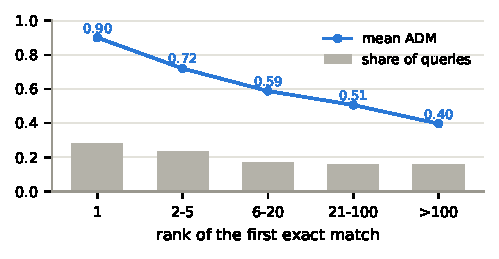
\includegraphics[width=\linewidth]{difficulty.pdf}
\caption{Per-query ADM against the rank of the first exact match (distilled ViT-L, PETA held out). Bars: share of queries per bin.}
\label{fig:difficulty}
\end{figure}

The likelihood score has one property that shapes the rest of this paper. A single confident error is very costly: $p=0.999$ on a wrong attribute subtracts 6.9 nats, enough to push an exact match far down the list. Retrieval under \cref{eq:ll} therefore depends on the whole probability vector, not only on which side of 0.5 each value falls. \Cref{sec:select} asks what this implies for model selection, and \cref{sec:train} for training.

%=====================================================================
\section{What the Score Rewards}
\label{sec:select}

Averaging \cref{eq:ll} over the exact matches of every query gives the negative log-likelihood (NLL) of the held-out label vectors, in nats per image summed over 40 attributes. NLL is therefore the natural model-selection criterion for this score. It is incomplete, though, because ranking depends on the margin between a match and its competitors, which NLL does not see. A criterion that does is the listwise log-likelihood: the log of the softmax of $s_{LL}$ over the gallery, averaged over the exact matches.

\Cref{fig:nll} tests the three criteria on the 41 PETA-held-out runs. Across all runs, mADM follows AUC moderately (Spearman $\rho=+0.73$), NLL strongly ($-0.94$) and the listwise criterion most closely ($+0.97$). Much of the AUC correlation comes from the encoder: ViT-L models have both higher AUC and higher mADM. Within the 14 B-size runs the picture separates. AUC has no predictive value ($\rho=-0.21$), the three Track~1 readouts of thresholded accuracy have none either ($-0.11$ to $+0.05$), while NLL ($-0.86$) and the listwise criterion ($+0.89$) still predict well.

\begin{figure*}[t]
\centering
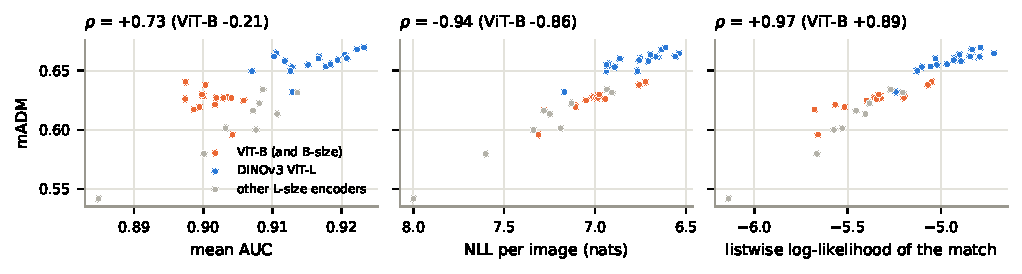
\includegraphics[width=\linewidth]{nll.pdf}
\caption{mADM against three selection criteria for the 41 PETA-held-out runs. Titles give Spearman's $\rho$ over all runs and over the 14 B-size runs. NLL axis reversed so that better is to the right in every panel.}
\label{fig:nll}
\end{figure*}

This changes design decisions. Our first retrieval system was selected with the Track~1 criterion, which saw no benefit in group cross-entropy (\cref{sec:train}): on the seed-matched ViT-B pair it changes thresholded accuracy by $-$0.00\pts\ under fitted offsets. On retrieval the same pair gains 1.20\pts\ mADM. Conversely, logit adjustment, which keeps AUC, multiplies NLL by about 4.6 in our earlier runs and lowers mADM by 8.6\pts.

%=====================================================================
\section{Calibration or Refinement?}
\label{sec:calib}

We now test the organizers' hypothesis directly. Following Kull and Flach~\cite{kull}, we split held-out NLL into a calibration term, the NLL that a per-attribute recalibration map $p=\sigma(a_kz+b_k)$ fitted on the same labels removes, and a refinement term, the NLL that remains. Fitting the map on the held-out labels is an oracle; fitting it on the validation data of the two source datasets is a usable method.

\begin{table}[t]
\centering\small
\setlength{\tabcolsep}{3pt}
\resizebox{\columnwidth}{!}{%
\begin{tabular}{@{}lccc@{}}
\toprule
& PETA & Market1501 & PA100k \\
\midrule
runs & 41 & 5 & 2 \\
held-out NLL (nats) & 6.97 & 6.09 & 9.38 \\
calibration term, held out & 1.29 & 1.10 & 3.88 \\
calibration term, source datasets & 1.10 & 0.89 & 3.74 \\
runs with held-out term larger & 37/41 & 5/5 & 2/2 \\
\midrule
$\Delta$mADM, oracle recalibration & +2.64 & +1.75 & +5.73 \\
$\Delta$mADM, source recalibration & $-$0.86 & $-$0.53 & +3.63 \\
runs where source recalibration helps & 0/41 & 0/5 & 1/2 \\
\midrule
NLL after: source scale + source bias & 6.60 & 5.87 & 6.10 \\
\phantom{NLL after:} source scale + held-out bias & 6.18 & 5.12 & 5.88 \\
\phantom{NLL after:} held-out scale + source bias & 6.55 & 5.85 & 8.19 \\
\phantom{NLL after:} held-out scale + held-out bias & 5.68 & 4.99 & 5.51 \\
\bottomrule
\end{tabular}}
\caption{Calibration on held-out and source data (means over runs). The map is $\sigma(a_kz+b_k)$ per attribute; ``scale'' is $a_k$, ``bias'' is $b_k$. The last row is the oracle.}
\label{tab:calib}
\end{table}

\paragraph{Miscalibration is real.} \Cref{tab:calib} shows that the oracle map recovers 2.64\pts\ of mADM on PETA, 1.75 on Market1501 and 5.73 on PA100k. This is more than any recognizer change in \cref{sec:train}, so the organizers are right that confidence quality limits retrieval.

\paragraph{But it is mostly not caused by the new domain.} The calibration term on the source datasets' own validation data is already 1.10 nats on the PETA fold, against 1.29 on the held-out data. The held-out term is larger in 44 of 48 runs, but the excess is only 3--19\% of the total. Most of the miscalibration is therefore built in by training: the targets are smoothed to 0.025 and 0.975 and the loss is weighted per attribute, so the network is not trained to output frequencies. The fitted scale $a_k$ has a median of 1.12 on both the source and the held-out data of the PETA fold, so in both domains the network is a little too soft by the same amount.

\paragraph{And the part that differs does not transfer.} If the miscalibration were the same in both domains, a map fitted on source data would fix most of it. It lowers held-out NLL (6.97 to 6.60 nats on PETA) but lowers mADM in 47 of 48 runs. The exception is the linear-head PA100k model, the worst calibrated of all. The last block of \cref{tab:calib} locates the failure by swapping the two parameters of the map. Using the source scale with the held-out bias recovers 61\% of the oracle's NLL reduction on PETA, 88\% on Market1501 and 90\% on PA100k. Using the held-out scale with the source bias recovers only 33\%, 22\% and 31\%. The scale transfers across domains and the per-attribute bias does not. This mirrors the Track~1 finding that per-attribute decision offsets fitted on source data do not transfer~\cite{track1}, and it explains why the organizers' diagnosis does not lead to a post-hoc fix.

Why does a map that lowers NLL lower mADM? NLL measures the probability of each image's own label vector, whereas ranking depends on how that probability compares with those of competing images. A per-attribute bias fitted on the wrong domain moves the score of every gallery image for that attribute, which can reorder matches and competitors even while each match's own probability rises. This is the gap between the NLL and listwise criteria of \cref{sec:select}.

\paragraph{Temperature.} A shared temperature is the most constrained map, and it also fails to transfer (\cref{fig:temp}). On PETA and Market1501 mild softening helps by up to 0.4\pts, while on PA100k every $T>1$ hurts, by 1.34\pts\ at $T=1.3$. Because \cref{eq:ll} sums log-probabilities over attributes, a temperature also changes the relative weight of confident and uncertain attributes, and so changes the ranking, not only the calibration. The best weighting differs by domain. Weighting each attribute by its source AUC~\cite{specker21} does not help on any domain (\cref{tab:scores}). We did not reproduce the full distribution-based distance of~\cite{specker21}. We therefore rank with the raw $s_{LL}$.

\begin{figure}[t]
\centering
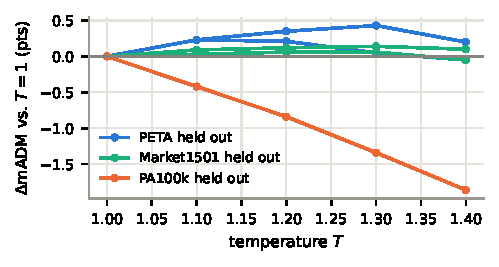
\includegraphics[width=\linewidth]{temperature.pdf}
\caption{Temperature scaling on three held-out domains (five model--domain pairs; PA100k has one model). No temperature helps every domain.}
\label{fig:temp}
\end{figure}

\begin{table}[t]
\centering\small
\setlength{\tabcolsep}{3pt}
\begin{tabular}{@{}lccc@{}}
\toprule
$\Delta$mADM vs.\ $s_{LL}$ (pts) & PETA & Market & PA100k \\
\midrule
$T=1.1$ & +0.23 & +0.03--0.09 & $-$0.42 \\
$T=1.3$ & +0.05--0.43 & +0.06--0.14 & $-$1.34 \\
AUC weights & 0.00 & +0.02 & $-$0.40 \\
squared AUC weights & $-$0.19 & $-$0.03 & $-$0.95 \\
expected ndom, weight 0.5 & +0.29 & not run & not run \\
softmax within groups & $-$0.5 to $-$1.2 & not run & not run \\
\bottomrule
\end{tabular}
\caption{Score-level variants. None improves every held-out domain.}
\label{tab:scores}
\end{table}

%=====================================================================
\section{Training for Held-Out Likelihood}
\label{sec:train}

If calibration fitted on source data cannot be corrected afterwards, the remaining lever is training. We examine three training choices and ask which part of the likelihood each one improves.

\paragraph{Group cross-entropy.} Age, hair length, lower-body type and the two 12-way color groups are mutually exclusive by definition. Independent sigmoids still spread probability over impossible combinations, such as two ages. For every group with exactly one positive $c$ we add $-\log\big(e^{z_c}/\sum_{k\in\mathcal G}e^{z_k}\big)$ to the loss with weight 0.5; samples without exactly one positive are skipped (11.7\% of PETA upper-color labels, which sometimes name two colors, and 12.2\% of PA100k hair labels). Inference still uses independent sigmoids.

\begin{table}[t]
\centering\small
\setlength{\tabcolsep}{2.5pt}
\resizebox{\columnwidth}{!}{%
\begin{tabular}{@{}llcccccc@{}}
\toprule
Held out & Base model & $\Delta$mADM & $\Delta$NLL & $\Delta$cal. & $\Delta$ref. & $\Delta$mADM$_{\text{or}}$ & $\Delta$AUC \\
\midrule
PETA & ViT-B query (seed 2) & +1.20 & $-$0.27 & $-$0.21 & $-$0.06 & +0.28 & $-$0.26 \\
PETA & ViT-B query, noise adaptation & +0.80 & $-$0.22 & $-$0.18 & $-$0.04 & +0.22 & +0.05 \\
PETA & ViT-B query, noisy-label mask & +0.40 & $-$0.17 & $-$0.15 & $-$0.02 & +0.19 & +0.30 \\
PETA & ViT-L query, 5 ep & +1.25 & $-$0.21 & $-$0.18 & $-$0.02 & +0.42 & +0.32 \\
PETA & ViT-L linear, 5 ep & +0.67 & $-$0.17 & $-$0.18 & +0.02 & +0.15 & $-$0.12 \\
PETA & ViT-L query, 3 ep & +0.84 & $-$0.24 & $-$0.23 & $-$0.01 & +0.14 & +0.39 \\
Market & ViT-B query & +0.56 & $-$0.14 & $-$0.03 & $-$0.11 & +0.36 & $-$0.15 \\
Market & ViT-B query, noise adaptation & +0.62 & $-$0.11 & $-$0.01 & $-$0.10 & +0.23 & +0.32 \\
\bottomrule
\end{tabular}}
\caption{Group cross-entropy, eight pairs that differ only in this loss. NLL and its calibration (cal.) and refinement (ref.) terms in nats; mADM$_{\text{or}}$ is mADM after oracle recalibration; mADM and AUC in points.}
\label{tab:gce}
\end{table}

\Cref{tab:gce} lists every pair of runs that differs only in this loss. mADM improves in all eight, by 0.40--1.25\pts, while AUC moves in both directions. The decomposition shows two different mechanisms. On PETA, nearly all of the NLL reduction is in the calibration term, and after oracle recalibration the gain shrinks to 0.14--0.42\pts. Group cross-entropy therefore improves held-out calibration, and it does so where post-hoc maps could not: in the six PETA pairs the held-out calibration term falls by 0.15--0.23 nats while the source term barely moves, which removes most of the held-out excess identified in \cref{sec:calib} (from 0.16--0.35 to $-$0.06--0.19 nats). On Market1501 the reduction is in refinement instead. We do not have a tested explanation for the PETA effect. One hypothesis is that the softmax ties the logits within a group together, so a domain-wide shift of one class (for example, a color cast raising every ``grey'' logit) must compete with the other classes instead of moving freely. \Cref{fig:nllg} shows where the NLL falls on PETA. Scoring with a softmax within groups at test time instead hurts by 0.5--1.2\pts\ (\cref{tab:scores}), plausibly because it forces exactly one positive per group on images whose labels have two or none.

\begin{figure}[t]
\centering
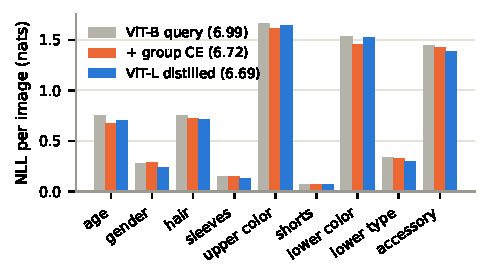
\includegraphics[width=\linewidth]{nll_groups.pdf}
\caption{Held-out NLL per image by attribute group on PETA, for a seed-matched pair without and with group cross-entropy and for a distilled ViT-L (totals in the legend).}
\label{fig:nllg}
\end{figure}

\paragraph{Label smoothing.} \Cref{sec:score} showed that a single confident error can bury an exact match. Smoothing the targets to 0.025 and 0.975 discourages such errors. Smoothing does not bound the outputs, but empirically it nearly does: across the 48 runs, at most 0.52\% of held-out cells give the true label a probability below 0.025, and at most 0.05\% below 0.01. As a sensitivity check, undoing the smoothing on trained logits (mapping each probability back as if the targets had been 0 and 1) lowers PETA mADM by 2.71\pts. This is not a training ablation, which we did not run; it shows only that the score depends strongly on the probability floor that smoothing produces.

\paragraph{Distillation.} We distil from the mean logits of DINOv3-L and CLIP-L teachers with weight 0.8 (\cite{track1} gives the details). \Cref{tab:kd} separates the effect of the teachers from that of training length on a ViT-L student. At equal length (3 epochs) distillation improves refinement by 0.06 nats and mADM by 0.40\pts, about one and a half standard errors, and after oracle recalibration the two are equal. Training longer without teachers makes refinement worse (5.51 to 5.58 nats from 3 to 5 epochs). With teachers it keeps improving, to 5.41 nats at 10 epochs, and mADM after recalibration rises by 1.2\pts. Distillation thus acts on refinement and makes longer training useful, in line with the Track~1 finding that the distilled student's AUC keeps rising with length.

\begin{table}[t]
\centering\small
\setlength{\tabcolsep}{3pt}
\resizebox{\columnwidth}{!}{%
\begin{tabular}{@{}lcccccc@{}}
\toprule
ViT-L 176 student & ep & mADM & NLL & cal. & ref. & mADM$_{\text{or}}$ \\
\midrule
label only (2 runs) & 3 & 65.15 & 6.91 & 1.40 & 5.51 & 67.83 \\
label only & 5 & 64.96 & 6.77 & 1.19 & 5.58 & 67.40 \\
DINOv3-L + CLIP-L & 3 & 65.55 & 6.93 & 1.47 & 5.46 & 67.89 \\
DINOv3-L + CLIP-L & 6 & 66.35 & 6.69 & 1.26 & 5.43 & 68.46 \\
DINOv3-L + CLIP-L & 10 & 66.81 & 6.63 & 1.22 & 5.41 & 69.06 \\
DINOv3-L + MetaCLIP2-H & 10 & 66.97 & 6.61 & 1.22 & 5.40 & 68.87 \\
\bottomrule
\end{tabular}}
\caption{Distillation and training length (PETA held out, no group cross-entropy). mADM in points, NLL terms in nats.}
\label{tab:kd}
\end{table}

For the ViT-B used at test time, two-teacher distillation with mixed inputs (function matching~\cite{patient}) for 10 epochs raises PETA mADM from 64.06 (group cross-entropy, 5 epochs) to 65.77, close to an undistilled ViT-L with group cross-entropy (66.22). The comparison is confounded by training length, so we read it only as ``distillation closes most of the B-to-L gap''.

%=====================================================================
\section{Hidden-Test Results}
\label{sec:lb}

\begin{table}[t]
\centering\small
\setlength{\tabcolsep}{3.5pt}
\begin{tabular}{@{}llc@{}}
\toprule
& Changes from the previous row & mADM \\
\midrule
v3b & ViT-B query head, group CE, $s_{LL}$ & 62.47 \\
v5 & + two-teacher distillation, 10 epochs & 63.15 \\
v6 & + mixed inputs, 20 epochs & \textbf{63.65} \\
\bottomrule
\end{tabular}
\caption{Hidden-test submissions (values $\times100$).}
\label{tab:main}
\end{table}

\Cref{tab:main} lists the submissions with recorded scores. Each step changes two factors, so we do not attribute the gains to single causes. Both steps are positive and exceed the replicate noise of \cref{sec:task}, and their direction agrees with \cref{tab:kd}. The organizers' 2027 baseline score was not available to us, so we cannot say by how much the system beats it.

%=====================================================================
\section{Discussion}
\label{sec:disc}

\paragraph{The answer to the title.} Partly. Miscalibration costs 1.8--5.7\pts\ of mADM on held-out data, more than any training change we found, so the organizers' diagnosis identifies a real loss. But it is not mainly created by the domain shift, and the part that the shift adds is a per-attribute bias that source data cannot estimate. What a designer can act on is the training signal: a loss that respects exclusive groups, which reduces the shift-specific miscalibration on PETA, and distillation with a long schedule, which improves refinement. Selecting these changes requires held-out likelihood, not thresholded accuracy or AUC.

\paragraph{Information we chose not to use.} Test queries are the distinct label vectors of the test gallery, so statistics across queries are statistics of test labels. On validation, two such tricks add 0.2--0.5\pts\ mADM; one is dropping the six colors that Market1501 never labels. We use neither, nor gallery-level re-ranking~\cite{kreciprocal}, because the challenge rules forbid using test information beyond the inputs of each query.

\paragraph{Limitations.} Most runs hold out PETA, and PA100k has only two. Label smoothing was not ablated in training. Distillation comparisons for ViT-B are confounded by length. \Cref{eq:ll} assumes attributes are independent given the image, which group cross-entropy deliberately violates during training. We did not compare against the full method of~\cite{specker21} or the organizers' 2027 baseline.

\paragraph{Broader impact.} Retrieving people by attributes such as age and gender in surveillance video can enable tracking of individuals without their consent. We report technical findings only and do not release trained models.

\section{Conclusion}

On unseen cameras, rank by the likelihood of the exact query and select models by held-out likelihood. Expect a large calibration loss that cannot be fixed with source data, because its domain-specific part is a per-attribute bias. Reduce it, and improve refinement, through the training signal instead.

{\small
\begin{thebibliography}{99}\setlength{\itemsep}{0pt}
\bibitem{upar} A.~Specker, M.~Cormier, J.~Beyerer. UPAR: Unified pedestrian attribute recognition and person retrieval. In \textit{WACV}, 2023.
\bibitem{upar23} M.~Cormier \etal. UPAR challenge: Pedestrian attribute recognition and attribute-based person retrieval -- dataset, design, and results. In \textit{WACV Workshops}, 2023.
\bibitem{upar24} M.~Cormier \etal. UPAR challenge 2024: Pedestrian attribute recognition and attribute-based person retrieval -- dataset, design, and results. In \textit{WACV Workshops}, 2024.
\bibitem{track1} Anonymous. Ranking transfers, thresholds do not: Diagnosing cross-domain pedestrian attribute recognition. UPAR Challenge 2027, Track 1 technical report.
\bibitem{vaquero} D.~A.~Vaquero, R.~S.~Feris, D.~Tran, L.~Brown, A.~Hampapur, M.~Turk. Attribute-based people search in surveillance environments. In \textit{WACV}, 2009.
\bibitem{siddiquie} B.~Siddiquie, R.~S.~Feris, L.~S.~Davis. Image ranking and retrieval based on multi-attribute queries. In \textit{CVPR}, 2011.
\bibitem{dap} C.~H.~Lampert, H.~Nickisch, S.~Harmeling. Learning to detect unseen object classes by between-class attribute transfer. In \textit{CVPR}, 2009.
\bibitem{specker21} A.~Specker, J.~Beyerer. Improving attribute-based person retrieval by using a calibrated, weighted, and distribution-based distance metric. In \textit{ICIP}, 2021.
\bibitem{specker23} A.~Specker, J.~Beyerer. Balanced pedestrian attribute recognition for improved attribute-based person retrieval. In \textit{ICPRS}, 2023.
\bibitem{pa100k} X.~Liu \etal. HydraPlus-Net: Attentive deep features for pedestrian analysis. In \textit{ICCV}, 2017.
\bibitem{market} L.~Zheng \etal. Scalable person re-identification: A benchmark. In \textit{ICCV}, 2015.
\bibitem{peta} Y.~Deng, P.~Luo, C.~C.~Loy, X.~Tang. Pedestrian attribute recognition at far distance. In \textit{ACM MM}, 2014.
\bibitem{prp} S.~E.~Robertson. The probability ranking principle in IR. \textit{Journal of Documentation}, 1977.
\bibitem{gneiting} T.~Gneiting, A.~E.~Raftery. Strictly proper scoring rules, prediction, and estimation. \textit{JASA}, 2007.
\bibitem{gneitingsharp} T.~Gneiting, F.~Balabdaoui, A.~E.~Raftery. Probabilistic forecasts, calibration and sharpness. \textit{JRSS-B}, 2007.
\bibitem{degroot} M.~H.~DeGroot, S.~E.~Fienberg. The comparison and evaluation of forecasters. \textit{The Statistician}, 1983.
\bibitem{brocker} J.~Br\"ocker. Reliability, sufficiency, and the decomposition of proper scores. \textit{Quarterly Journal of the Royal Meteorological Society}, 2009.
\bibitem{kull} M.~Kull, P.~Flach. Novel decompositions of proper scoring rules for classification: Score adjustment as precursor to calibration. In \textit{ECML-PKDD}, 2015.
\bibitem{guo} C.~Guo, G.~Pleiss, Y.~Sun, K.~Q.~Weinberger. On calibration of modern neural networks. In \textit{ICML}, 2017.
\bibitem{ovadia} Y.~Ovadia \etal. Can you trust your model's uncertainty? Evaluating predictive uncertainty under dataset shift. In \textit{NeurIPS}, 2019.
\bibitem{muller} R.~M\"uller, S.~Kornblith, G.~Hinton. When does label smoothing help? In \textit{NeurIPS}, 2019.
\bibitem{hinton} G.~Hinton, O.~Vinyals, J.~Dean. Distilling the knowledge in a neural network. \textit{arXiv:1503.02531}, 2015.
\bibitem{patient} L.~Beyer \etal. Knowledge distillation: A good teacher is patient and consistent. In \textit{CVPR}, 2022.
\bibitem{kreciprocal} Z.~Zhong, L.~Zheng, D.~Cao, S.~Li. Re-ranking person re-identification with k-reciprocal encoding. In \textit{CVPR}, 2017.
\bibitem{dinov3} O.~Sim\'eoni \etal. DINOv3. \textit{arXiv:2508.10104}, 2025.
\end{thebibliography}
}

\clearpage
\appendix
\onecolumn
\section{Where rankings go wrong}

\begin{figure}[h]
\centering
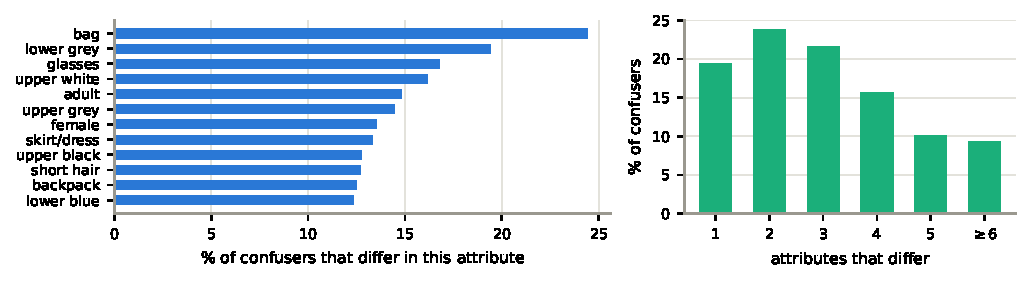
\includegraphics[width=0.9\linewidth]{confusers.pdf}
\caption{Non-matching images ranked above the first exact match (up to ten per query; distilled ViT-L, PETA held out). Left: the attributes they most often get wrong; small accessories and neutral colors dominate. Right: how many attributes are wrong. 43\% differ in one or two attributes and still earn most of the near-miss credit.}
\end{figure}

\section{Implementation}
\label{app:impl}

The submission predicts 40 probabilities per gallery image and clips them to $[10^{-4},1-10^{-4}]$. It forms $L^+=\log P$ and $L^-=\log(1-P)$, computes $S=Q(L^+-L^-)^\top+\mathbf 1(L^-\mathbf 1)^\top$ in float64, casts it to float32, and returns $-S$ as the distance matrix expected by the organizers' code. For about 3{,}500 queries and 29k images one float64 matrix takes 0.8\,GB.

The expected-ndom variant of \cref{tab:scores} uses the per-attribute error probability $m_k=q_k(1-p_k)+(1-q_k)p_k$ and $r_k=m_k/(1-m_k)$. The power sums $P_t=\sum_kr_k^t$ are matrix products, Newton's identities turn them into elementary symmetric polynomials $e_j$, and the probability of exactly $j$ wrong attributes is $e^{s_{LL}}e_j$.

Recalibration maps are per-attribute logistic regressions on the logit (scikit-learn, $C=10^4$). The listwise criterion is $\frac1{|Q|}\sum_q\frac1{R_q}\sum_{g\in\text{matches}(q)}\big[s_{LL}(q,g)-\log\sum_{g'}e^{s_{LL}(q,g')}\big]$. Training follows Track~1: AdamW, learning rate $5\cdot10^{-5}$ with layer decay 0.75, batch 64, cosine schedule, EMA 0.9995, label smoothing 0.05 and DeepMAR weights.

\end{document}
